\documentclass[letterpaper,11pt]{notes}


%%%%%%%%%%%%%%%%%%%%%%%%%%%%%%%%%%%%%%%%%%%%%%%%%%%%%%%%%%%%%%%%%%%%%%%%%%%%%%%%%%%%%%%%%%%%%%
%%%%%%%%%%%%%%%%%%%%%%%%%%%%%%%%%%%%%%%%%%%%%%%%%%%%%%%%%%%%%%%%%%%%%%%%%%%%%%%%%%%%%%%%%%%%%%
%%%%%%%%%%%%%%%%%%%%%%%%%%%%%%%%%%%%%%% WARNING %%%%%%%%%%%%%%%%%%%%%%%%%%%%%%%%%%%%%%%%%%%%%%
% The following is here just to demonstrate the nofancy option for this template, and should be removed in any real document
\theoremstyle{definition}
\newtheorem{dfn}{Definition}[section]
\newtheorem{Iexm}{Example}[section]
   
\theoremstyle{plain}
\newtheorem{Ithm}{Theorem}[section]
\newtheorem{Ilem}{Lemma}[section]

\newenvironment{definitionA}[2]
    {\begin{dfn}[#1]\ifstrempty{#2}{}{\label{dfnA:#2}}}
    {\end{dfn}}
\newenvironment{lemA}[2]
    {\begin{Ilem}[#1]\ifstrempty{#2}{}{\label{lemA:#2}}}
    {\end{Ilem}}
\newenvironment{thmA}[2]
    {\begin{Ithm}[#1]\ifstrempty{#2}{}{\label{thmA:#2}}}
    {\end{Ithm}}
\newenvironment{exampleA}[2]
    {\begin{Iexm}[#1]\ifstrempty{#2}{}{\label{exmA:#2}}}
    {\end{Iexm}}
    
\theoremstyle{remark}
\newtheorem*{proofA}{Proof}
%%%%%%%%%%%%%%%%%%%%%%%%%%%%%%%%%%%%%%%%%%%%%%%%%%%%%%%%%%%%%%%%%%%%%%%%%%%%%%%%%%%%%%%%%%%%%%
%%%%%%%%%%%%%%%%%%%%%%%%%%%%%%%%%%%%%%%%%%%%%%%%%%%%%%%%%%%%%%%%%%%%%%%%%%%%%%%%%%%%%%%%%%%%%%

\title{Notes template}
\author{Tadej Svetina\thanks{\tt tadej@mit.edu}\\MIT}
\date{June 2019}

\begin{document}

\maketitle

\section{Introduction}

This is a sample document using the custom \texttt{notes} class (with the \texttt{macros} package). The primary aim of the \texttt{notes} class is to move all the boilerplate usually found in the preamble of the \texttt{main.tex} file to a reusable class file, making the actual document code shorter and easier to read.

Complementing that, the secondary aim of the \texttt{notes} class and the \texttt{macros} package is to create short commands for some frequently used things, cutting down on typing/tinkering time and improving readability.

Finally, as we have a reusable class and package, we might as well define some nice looking defaults. For this purpose, the class/package define (or show)
\begin{itemize}
    \item a custom color palette, based on \href{https://personal.sron.nl/~pault/}{Paul Tol's vibrant scheme}
    \item nice fancy theorem environments (optional),
\end{itemize}

I showcase all of the above mentioned features in this template, and as a bonus, also how to get easy code highlighting in \LaTeX, how to typset nice tables with \texttt{booktabs} and how to adjust fonts and colors for python graphs to match the document. 

Finally, to use the class/package combo, just put both files in the root project repository, and add the following line to the top of the \texttt{main.tex} file
\begin{minted}{latex}
\documentclass{notes}
\end{minted}
Nothing else is needed!

\section{Class options}
The \texttt{notes} class defines the following class-specific options:
\begin{itemize}
    \item \texttt{letterpaper}: Sets the paper size to letter paper, with 1 inch margins. This is the default.  
    \item \texttt{a4paper}: Sets the paper size to A4 paper, with 1 inch margins.  
    \item \texttt{a5paper}: Sets the paper size to A5 paper, with $0.75$ inch margins.  
    \item \texttt{b5paper}: Sets the paper size to B5 paper, with $0.75$ inch margins.  
    \item \texttt{nofancy}: This removes the fancy formatting from the theorem environments, giving them the standard \texttt{amsthm} formatting, see section \ref{nofancy}.  
\end{itemize}

Any other options passed to \texttt{notes} class will simply be passed to the \texttt{article} class, on which \texttt{notes} builds.

\section{Colors} \label{colors}
The color palette defines the following colors (which are obtained by \texttt{m} + capitalized name of the color):
\begin{itemize}\bfseries
    \item \textcolor{mBlue}{blue,} \textcolor{mCyan}{cyan,} \textcolor{mTeal}{teal,} \textcolor{mOrange}{orange,} \textcolor{mRed}{red,} \textcolor{mMagneta}{magneta,} \textcolor{mGrey}{grey} 
\end{itemize}

There are two commands that use these colors: \texttt{\alert{\textbackslash{}alert}} and \texttt{\define{\textbackslash{}define}}.

\section{Theorems}

The only special custom thing are the theorems, which are (by default) made "fancy" with the \texttt{tcolorbox} environment. This can be turned off by passing \texttt{nofancy} option to the document class. The following theorem-environments are supported:
\begin{itemize}
    \item Theorem (\texttt{thm})
    \item Lemma (\texttt{lem})
    \item Example (\texttt{exm})
    \item Definition (\texttt{definition})
\end{itemize}
Additionally, \texttt{proof} also has a fancy version with a colorful frame, but it is not numbered.


\subsection{Theorem}
The following example shows the basic syntax of the \texttt{thm} command:
\begin{minted}{latex}
\begin{thm}{Cauchy-Schwarz inequality}{cs}
    For all vectors $\vec{u}$ and $\vec{v}$ in ...
\end{thm}
\end{minted}
Output of this command is:

\begin{thm}{Cauchy-Bunyakovsky-Schwarz inequality}{cs}
For all vectors $\vec{u}$ and $\vec{v}$ in an inner product space it is true that
\begin{equation}
    \left|\langle\vec{u}, \vec{v}\rangle\right|^2 \leq \langle\vec{u}, \vec{u} \rangle \cdot \langle\vec{v}, \vec{v} \rangle 
\end{equation}
\end{thm}

\subsection{Lemma}
The following example shows the basic syntax of the \texttt{lem} command:
\begin{minted}{latex}
\begin{lem}{Titu's Lemma}{titu}
    For some $u_i, v_i \in \Rnn$, it is true that ...
\end{lem}
\end{minted}
Output of this command is:
\begin{lem}{Titu's Lemma}{titu}
For some $u_i, v_i \in \Rnn$, it is true that
\begin{equation}
    \frac{\left(\si u_i\right)^2}{\si v_i} \leq \si \frac{u_i^2}{v_i}
\end{equation}
\end{lem}

\subsection{Proof}
The following example shows the basic syntax of the \texttt{proof} command, as well as how the references to the above Lemma and Theorem work.
\begin{minted}{latex}
\begin{proof}
    To prove Lemma \ref{lem:titu}, we just need to replace $u_i' = \frac{u_i}{\sqrt{v_i}}$ and $v_i' = \sqrt{v_i}$, and then apply Theorem \ref{thm:cs}. 
\end{proof}
\end{minted}
The output is:
\begin{proof}
To prove Lemma \ref{lem:titu}, we just need to replace $u_i' = \frac{u_i}{\sqrt{v_i}}$ and $v_i' = \sqrt{v_i}$, and then apply Theorem \ref{thm:cs}. 
\end{proof}

\subsection{Example and definition}
The syntax is basically the same as for Lemma and Proof, so I omit the code. Note the use of \texttt{define} command in the definition.

\begin{definition}{}{}
We say that a set $A$ is \define{closed}, if its complement $A^C$ is open.
\end{definition}

\begin{example}{}{}
In the discrete topology, the closed sets are $X$ and $\emptyset$.
\end{example}

\subsection{\texttt{nofancy} theorems} \label{nofancy}
Here we show how the previous examples in this section would have looked like if we passed the \texttt{nofancy} option to the document class. The code syntax would have remained the same, of course.

\begin{thmA}{Cauchy-Schwarz inequality}{cs}
For all vectors $\vec{u}$ and $\vec{v}$ in an inner product space it is true that
\begin{equation}
    \left|\langle\vec{u}, \vec{v}\rangle\right|^2 = \langle\vec{u}, \vec{u} \rangle \cdot \langle\vec{v}, \vec{v} \rangle 
\end{equation}
\end{thmA}

\begin{lemA}{Titu's Lemma}{titu}
For some $u_i, v_i \in \Rnn$, it is true that
\begin{equation}
    \frac{\left(\si u_i\right)^2}{\si v_i} \leq \si \frac{u_i^2}{v_i}
\end{equation}
\end{lemA}

\begin{proofA}
To prove Lemma \ref{lem:titu}, we just need to replace $u_i' = \frac{u_i}{\sqrt{v_i}}$ and $v_i' = \sqrt{v_i}$, and then apply Theorem \ref{thm:cs}. \hfill \qedsymbol % A bit of hacking here...
\end{proofA}

\begin{definitionA}{}{}
We say that a set $A$ is \define{closed}, if its complement $A^C$ is open.
\end{definitionA}

\begin{exampleA}{}{}
In the discrete topology, the closed sets are $X$ and $\emptyset$.
\end{exampleA}

\section{Tables}

The example bellow shows how to make a simple table using the \texttt{booktabs} package:

\begin{table}[H]
    \centering

    \begin{tabular}{@{}llr@{}}  
        \toprule
        \multicolumn{2}{c}{Item} \\
        \cmidrule(r){1-2}
        Animal    & Description & Price (\$) \\
        \midrule
        Gnat      & per gram    & 13.65      \\
                  &    each     & 0.01       \\
        Gnu       & stuffed     & 92.50      \\
        Emu       & stuffed     & 33.33      \\
        Armadillo & frozen      & 8.99       \\
        \bottomrule
    \end{tabular}
    
    \caption{Price list}
    \label{tab:my_label}
\end{table}


The code used to produce this example is
\inputminted{latex}{table.tex}

\section{Code}

This isn't anything special to the \texttt{notes} class, but I just show how to write beautifully formatted Python code for reference. Here is how some python code looks like:
\inputminted[linenos]{python}{code.py}%
We can make use of code separation and import the code to be displayed from a separate \texttt{.py} file, indeed, the previous example was produced by (\texttt{linenos} is used to add line numbers)
\begin{minted}{latex}
\inputminted[linenos]{python}{code.py}
\end{minted}
and the line of code above was produced with\footnote{In the example we wrote \texttt{m inted} instead of \texttt{minted}, as otherwise \texttt{\textbackslash{}end\{minted\}} is not properly escaped.}
\begin{minted}{latex}
\begin{m inted}{latex}
    \inputminted{python}{code.py}
\end{m inted}
\end{minted}

\section{Python graphs}

When trying to match the style of python (matplotlib) graphs, two main adjustments have to be considered: fonts and colors.

\subsection{Text width}

But even before that, another "adjustment" should be made: the dimensions of the figure should be set to be smaller than those of the document. The relevant dimension here is width, or to be precise \texttt{\textbackslash{}textwidth}. But the pure \LaTeX\ ways of getting this give us the size in points (and we need it in inches), so to get it we use the \texttt{printlen} package:
\begin{minted}{latex}
\uselengthunit{in}\printlength{\textwidth}
\end{minted}
As an example, the text width of this document is \uselengthunit{in}\printlength{\textwidth}.



\subsection{Fonts}

We need to make sure that the fonts in the document match the fonts in the graph. Matplotlib has a limited selection of fonts, so its safest to let \LaTeX\ do all the font processing. We need to load the fonts and change the size to match that of our document. We would do this by putting this at the beginning of our code
\begin{minted}{python}
from matplotlib import rc

rc('text.latex',preamble=r'\usepackage[charter, cal=cmcal]{mathdesign}')
rc('text',usetex=True)
rc('font', family='serif', size=11)
\end{minted}

Note that this will slow down processing quite a bit, so \alert{only change the fonts when the figures are done!}

\subsection{Colors}

We might also want to use our standard color palette (see section \ref{colors}) -- although this is more a matter of taste, there is nothing wrong with matplotlib color palettes. The way we would implement them is with
\begin{minted}{python}
from matplotlib import rc
from cycler import cycler

colors = ['#0077BB', '#EE7733', '#009988', '#CC3311', '#33BBEE', '#EE3377']
rc('axes', prop_cycle = cycler(c=colors))
\end{minted}


\subsection{An example}
Let's put the two things together, to create a simple example. Here is the code:
\inputminted[linenos]{python}{fig.py}%
The result is shown in Figure \ref{fig:trig}. To completely visually merge the figure in the document we would probably need to tweak a few more things (for example the legend box), but as far as the fonts and colors are concerned, we are done. Note that we set the width of the figure to 6 inches -- that's ok, as we have seen that the width of our document is \uselengthunit{in}\printlength{\textwidth}. 

There are also a few extra useful tweaks in the code:
\begin{itemize}
    \item The title size is set, in line 25, to the document size (11) -- this is because by default, the title size is a bit bigger (other graph elements do not have this problem). But this is most likely not relevant anyways, as you would not need a title on a figure that will already have a caption.
    \item The path in \texttt{savefig} (line 34) is set to the Overleaf Dropbox repository. This is a great way to get continuous updating with Overleaf every time you change the figure in the code, without having to manually copy/paste or git commit/push.
\end{itemize}

\begin{figure}
    \centering
    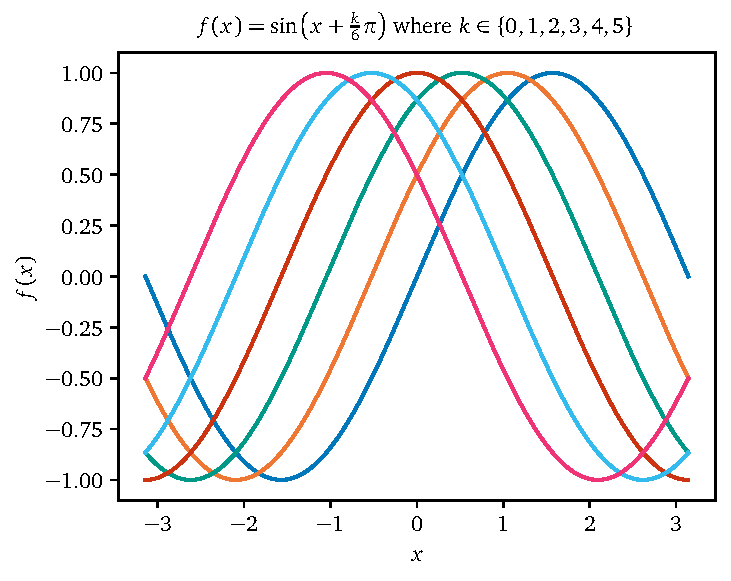
\includegraphics{trig.pdf}
    \caption{Some trigonometric functions}
    \label{fig:trig}
\end{figure}

\section{Todo}
There are a couple of things that I would like to add to this class (package), including
\begin{itemize}
    \item Macros for some commonly used list variations from the \texttt{enumitem} package
    \item Macros for multiline equations (\texttt{IEEEtrantools} based)
    \item Explore \texttt{captionof} package in conjunction with \texttt{tcolorbox} to include figures in theorem environments
    \item Tweak some spacing (after \texttt{minted}, between list items)
    \item Macros for easier table and figure input
\end{itemize}

\end{document}
